\documentclass[10pt,journal,compsoc]{styles/IEEEtran}
\usepackage{styles/algorithm}
\usepackage[noend]{styles/algorithmic}
\usepackage{graphicx}
\usepackage{color}
\usepackage{listings}
\usepackage{amsmath}
\usepackage[utf8]{inputenc}
\usepackage[T1]{fontenc}
\usepackage[labelformat=empty]{caption}
% *** CITATION PACKAGES ***
\ifCLASSOPTIONcompsoc
  % IEEE Computer Society needs nocompress option
  % requires cite.sty v4.0 or later (November 2003)
  \usepackage[noadjust]{cite}
\else
  % normal IEEE
  \usepackage{cite}
\fi

\title{Proyecto: Algoritmo Mem\'etico Aplicado a Optimizaci\'on Continua}

\author{Juan Gerardo Fuentes Almeida}

% The paper headers
\markboth{Algoritmo Mem\'etico Aplicado a Optimizaci\'on Continua}%
{Shell \MakeLowercase{\textit{et al.}}: Bare Advanced Demo of styles/IEEEtran.cls for Journals}

\IEEEtitleabstractindextext{%
\begin{abstract}
En este proyecto se implementa un algoritmo mem\'etico para optimización continua, aplicado a un problema de optimización de parámetros de un mecanismo de 4 brazos.
\end{abstract}
}

\begin{document}

% make the title area
\maketitle

\IEEEdisplaynontitleabstractindextext

\IEEEpeerreviewmaketitle

\section{Introducci\'on}

\IEEEPARstart{S}e dice que la cultura humana est\'a conformada por unidades de conocimiento denominadas \emph{memes}. Un meme es un bloque de conocimiento que puede ser duplicado en el cerebro humano y ser modificado o combinado con otros memes para generar nuevos. Dentro de un comunidad, algunos memes sencillamente no son interesantes y se extinguen en un periodo corto de tiempo; otros son m\'as bien resistentes y se propagan entre la comunidad entera, como si fuera una infección. También pueden experimentar ligeras modificaciones o combinarse entre ellos y asi generar nuevos memes con características mas resistentes y ser mas durables y propensos a propagarse.\\

Esta interpretación de la cultura humana inspir\'o a Moscato y Norman a finales de los 80's para definir los Algoritmos Mem\'eticos (MA's) como una modificación de los Algoritmos Genéticos (GA's) incluyendo una búsqueda local.\\

	
\section{Teoría}

El Algoritmo Mem\'etico Estándar se compone de los siguientes operadores:\\

	\begin{enumerate}
	\item Selección de padres.
	\item Combinación de los padres para generar descendencia.
	\item Mejoramiento local de la descendencia.
	\item Actualización de la población.
	\end{enumerate}

La estructura básica del Algoritmo Mem\'etico se muestra en el Algoritmo 1. Los procedimientos \emph{Cooperate}, \emph{Improve} y \emph{Compete} constituyen el núcleo principal del algoritmo, la función \emph{Cooperate} involucra a todos los individuos de la población para generar una descendencia que puede poseer rasgos ya sea de uno o varios padres. La función \emph{Improve} ejecuta una búsqueda local dentro de la nueva población generada, con el propósito de mejorar localmente la descendencia generada, mientras que la función \emph{Compete} realiza un proceso de selección entre la población nueva y la anterior para determinar los individuos que pasar\'an a la siguiente generación.

    \begin{figure}[H]
    \centering
    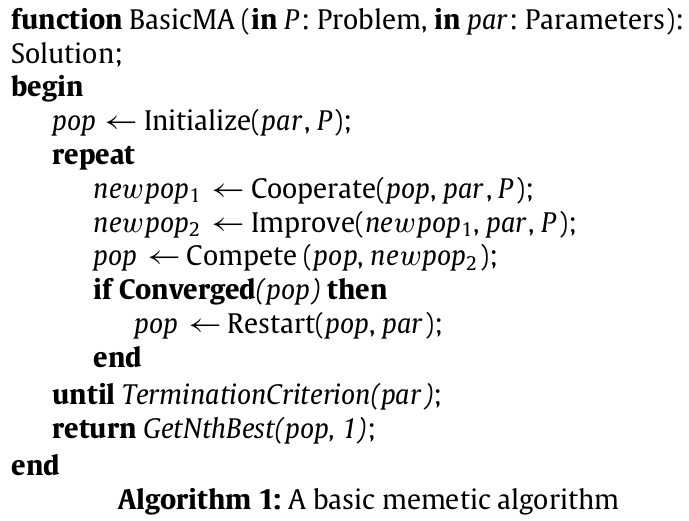
\includegraphics[width = 0.4\textwidth]{alg1.png}
    \caption{}
  	\end{figure}
  
El procedimiento de Inicialización, descrito en el Algoritmo 2, es el responsable de producir el conjunto inicial de $|pop|$ soluciones. Esto puede realizarse de manera aleatoria, pero típicamente en un Algoritmo Mem\'etico se intenta producir soluciones de alta calidad desde el inicio, ya sea aplicando alguna heurística constructiva o una búsqueda local para mejorar las soluciones aleatorias.\\

    \begin{figure}[H]
    \centering
    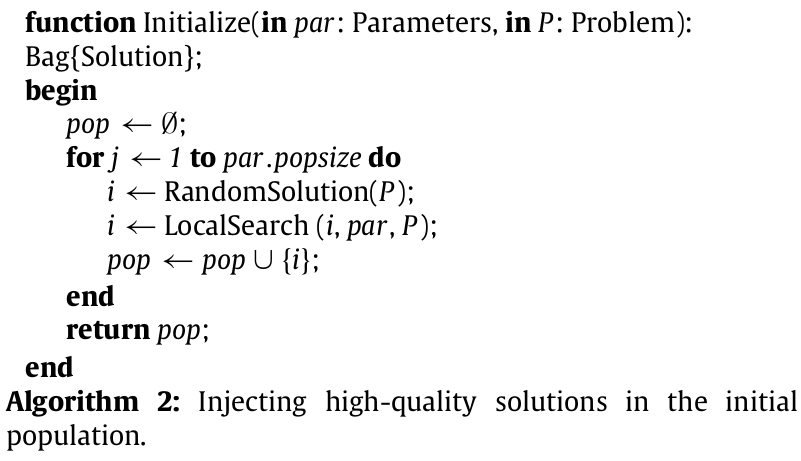
\includegraphics[width = 0.47\textwidth]{alg2.png}
    \caption{}
  	\end{figure}

La función \emph{Cooperate} (Algoritmo 3) parte de la utilización de dos operadores de selección de individuos de entre la población y recombinaci\'on entre ellos, pero también ser fácilmente extendido al uso de una colección mas grande de operadores de variación.\\

    \begin{figure}[H]
    \centering
    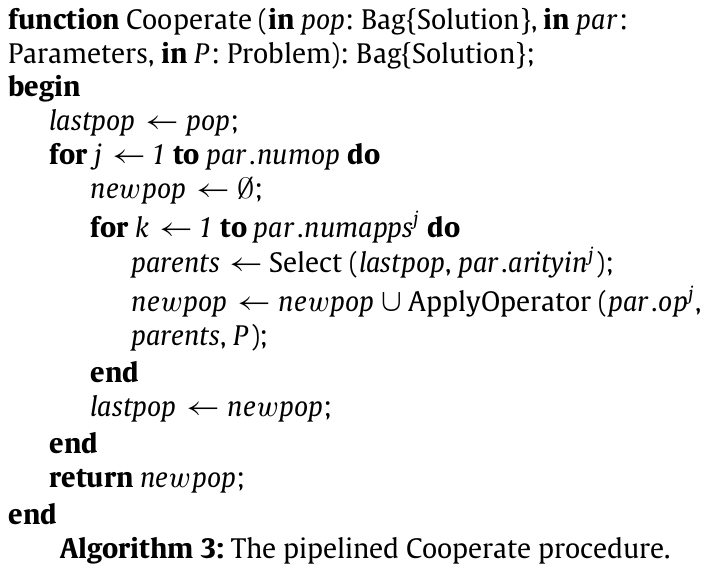
\includegraphics[width = 0.4\textwidth]{alg3.png}
    \caption{}
  	\end{figure}

El procedimiento de mejora incorpora la aplicacion de una busqueda local entre los individuos de la poblacion, teniendo en cuenta que para optimizacion continua, la vecindad $N(s)$ de una solucion $s$ es una hiperesfera con centro en $s$ y radio igual a $\epsilon$ con $\epsilon>0$.\\

Por tanto, se tiene que $N(s)=\{s' \in \Re^n : \parallel s'-s\parallel <\epsilon\}$ donde $\parallel s'-s\parallel$ es la norma Euclidiana.\\
  
    \begin{figure}[H]
    \centering
    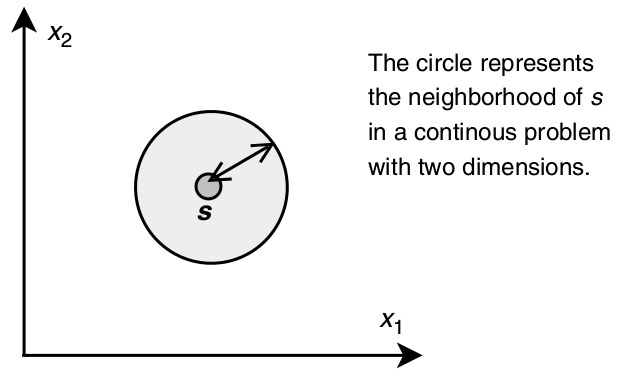
\includegraphics[width = 0.35\textwidth]{ls.png}
    \caption{Vecindad de una solución}
  	\end{figure}

Despues de realizar una serie de operadores, la poblacion generada $newpop2$ "compite" contra la poblacion anterior $pop$, construyendo asi una nueva poblacion a partir de estas dos. Existen dos posibles maneras de realizar este procedimiento, a saber, la estrategia \textit{Plus} y la estrategia \textit{Comma}:\\ 

	\begin{enumerate}
	\item Estrategia Plus: La nueva población es construida a partir de las mejores $popsize$ configuraciones de $pop \cup newpop$.\\
	\item Estrategia Comma: Las mejores $popsize$ configuraciones se toman solamente de $newpop$. En estos casos, se requiere que $|newpop| >popsize$ para incrementar la presión de selección del proceso.\\
	\end{enumerate}

En cuanto al procedimiento de reinicio, se debe decidir si la población se ha degradado o no, utilizando alguna medida de diversidad, tal como la desviación estándar en el caso de optimización continua o la entropía de Shannon en el caso discreto. Una estrategia típica de reemplazo consiste en conservar una fracción de la población actual y generar soluciones nuevas (de forma aleatoria o heurística) para completar el resto.\\

    \begin{figure}[H]
    \centering
    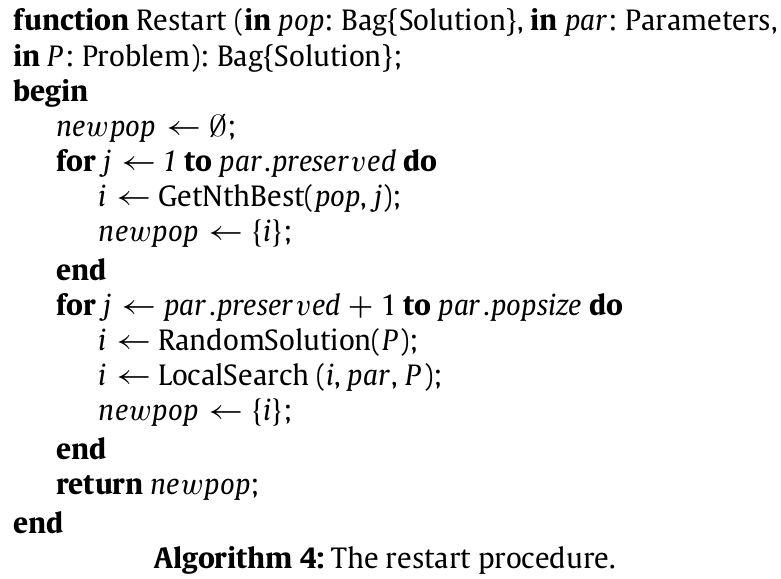
\includegraphics[width = 0.45\textwidth]{alg4.png}
    \caption{}
  	\end{figure}

El criterio de paro puede elegirse de entre cualquiera de estas opciones:

   \begin{enumerate}
   \item L\'imite en el numero total de iteraciones.
   \item Alcanzar un numero máximo de iteraciones sin ninguna mejora.
   \item Haber ejecutado un cierto numero de reinicios.
   \item Haber alcanzado un cierto valor de fitness.
   \end{enumerate}

\section{Descripci\'on del Problema}

\subsection{Mecanismo de cuatro brazos}

El objetivo es que la terminal $C$ alcance los mas posible a un conjunto de puntos de precision $\{C_d^i\}$. El par motriz est\'a asociado a $\theta_2$ mientras que $r_1,r_2,r_3,r_4,r_{cx},r_{cy},x_0,y_0$ y $\theta_0$ son parámetros de dise\~o a ser optimizados. Dados estos parámetros, es posible calcular las coordenadas de la terminal $C$.\\

   \begin{figure}[H]
    \centering
    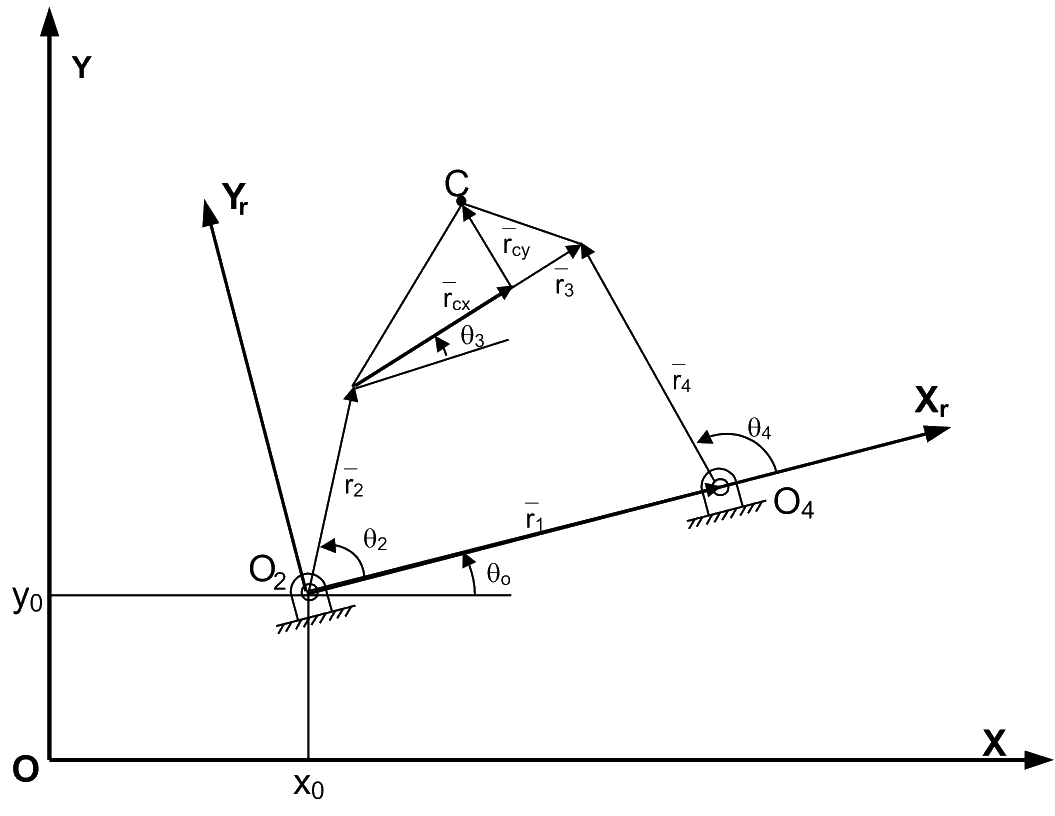
\includegraphics[width = 0.45\textwidth]{mecha.png}
    \caption{}
  \end{figure}
  
  
 Con respecto al sistema coordenado en $x_0$, $y_0$ y  $\theta_0$:
 
    $$\widehat{C}_r=\widehat{r}_2+\widehat{r}_{cx}+\widehat{r}_{cy}$$
    $$C_{xr}=r_2 \cos \theta_2 + r_{cx} \cos \theta_3 - r_{cy} \sin \theta_3$$
    $$C_{yr}=r_2 \sin \theta_2 + r_{cx} \sin \theta_3 + r_{cy} \cos \theta_3$$
    
Transformando al sistema coordenado \textbf{O}xy:

 	$$\begin{bmatrix}
 	C_x \\
 	C_y 
 	\end{bmatrix}=
 	\begin{bmatrix}
 	\cos \theta_0 & - \sin \theta_0 \\
 	\sin \theta_0 & \cos \theta_0
 	\end{bmatrix}
 	\begin{bmatrix}
 	C_{xr} \\
 	C_{yr} 
 	\end{bmatrix}+
 	\begin{bmatrix}
 	x_0 \\
 	y_0 
 	\end{bmatrix}$$

    Ecuación de lazo cerrado del mecanismo:
    
	$$\widehat{r}_1+\widehat{r}_4=\widehat{r}_2+\widehat{r}_3$$	
	$$r_2 \cos \theta_2 +r_3 \cos \theta_3=r_1 +r_4 \cos \theta_4$$
	$$r_2 \sin \theta_2 +r_3 \sin \theta_3=r_4 \sin \theta_4$$
	
	Elevando al cuadrado ambas ecuaciones:
	
	$$r_4^2 \cos^2 \theta_4=(r_2 \cos \theta_2 +r_3 \cos \theta_3-r_1)^2$$
	$$r_4^2 \sin^2 \theta_4=(r_2 \sin \theta_2 +r_3 \sin \theta_3)^2$$
	
	Sumando y aplicando identidades trigonométricas obtenemos:
 	$$r_4^2 = r_1^2 + r_2^2 + r_3^2 + 2r_2 r_3 \cos(\theta_2-\theta_3)- 2 r_1 r_3 \cos \theta_3 -2r_1 r_2 \cos \theta_2$$
  
	Reacomodando y redefiniendo los términos, formulamos la expresión conocida como \emph{Ecuación de Freudenstein}:
	
	$$k_1 \cos \theta_3 + k_2 \theta_2 + k_3 = \cos (\theta_2 - \theta_3)$$
	Donde:
	$$k_1=\frac{r_1}{r_2};~~ k_2=\frac{r_1}{r_3};~~ k_3=\frac{r_4^2-r_1^2 - r_2^2 - r_3^2}{2r_2 r_3}$$
	
Sea $\varphi=tan (\frac{\theta_3}{2})$, entonces
 
 $$\sin \theta_3 = \frac{2 \varphi}{1+\varphi^2};~~~ \cos \theta_3= \frac{1-\varphi^2}{1+\varphi^2}$$
 

 Sustituyendo en la ecuación de Freudenstein y reacomodando términos:
 
 $$k_1(\frac{1-\varphi^2}{1+\varphi^2})+ k_2 \cos \theta_2 + k_3 = (\frac{1-\varphi^2}{1+\varphi^2}) \cos \theta_2 + \frac{2 \varphi}{1+\varphi^2} \sin \theta_2$$
 
 \begin{footnotesize}
   $$\varphi^2[k_3+(k_2+1)\cos \theta_2 -k_1]+ \varphi(-2\cos \theta_2) + [k_1+(k_2-1)\cos \theta_2 + k_3]=0$$
 \end{footnotesize}


 
 Aplicando la formula cuadrática:
 
 $$\Rightarrow \varphi=\frac{-b\pm \sqrt{b^2-4ac}}{2a}$$

 Donde:

 $$a=k_3+(k_2+1)\cos \theta_2 -k_1$$
 $$b=-2\cos \theta_2$$
 $$c=k_1+(k_2-1)\cos \theta_2 + k_3$$

 Luego, $\theta_3$ puede ser calculado como $\theta_3=2tan^{-1} \varphi$\\

 Si $\varphi \not\in \Re$, el mecanismo no puede construirse con las configuraciones dadas.\\
 
\subsection{Restricciones}

 \begin{enumerate}
 \item Los \'angulos de entrada $\theta_2^i$ deben ser ordenados de modo que sean consecutivos en una circunferencia de $2\pi$ radianes.
 \item Todas las magnitudes de lo brazos deben ser positivas: $r_1,r_2,r_3,r_4,r_{cx},r_{cy}>0$.
 \item Se impone la condici\'on de Grashof para formar una configuraci\'on \emph{Crank-Rocker}, esto es $r_1+r_2<r_3+r_4$, con $r_2<r_3,r_4<r_1$, y el brazo m\'as corto conectado a la base.
   \begin{figure}[H]
    \centering
    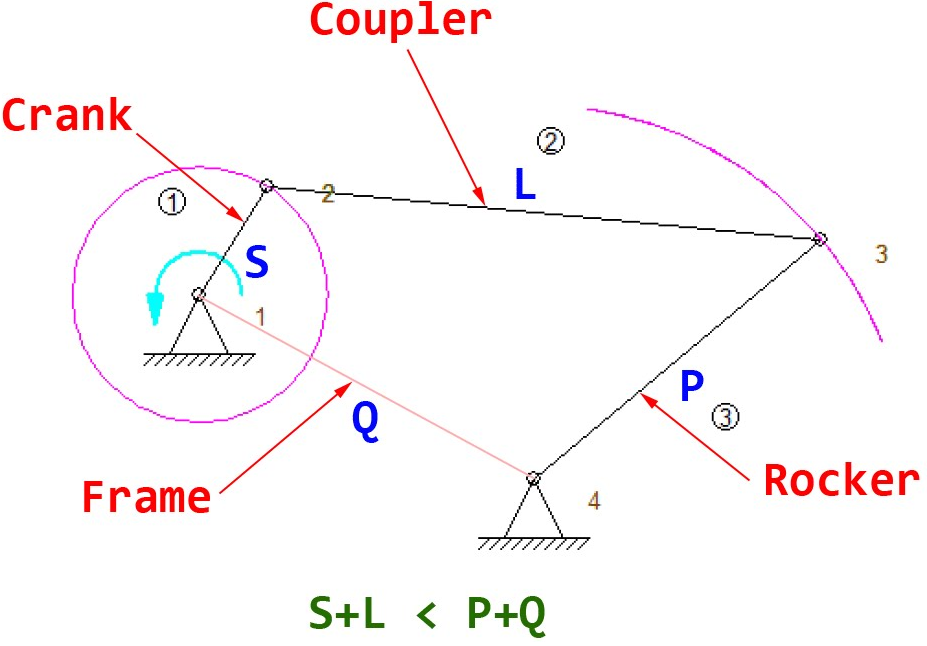
\includegraphics[width = 0.4\textwidth]{grashof.png}
    \caption{}
  \end{figure}

 \end{enumerate}
 

\section{Implementaci\'on}

\subsection{Funci\'on Objetivo}
Con base en la definici\'on del problema explicada anteriormente, el algoritmo de optimizaci\'on se implementa considerando las restricciones 1), 2) y 3) al asignar valores a las variables de dise\~no, es decir, se procura que los valores que toman las variables desde el inicio cumplan con estas condiciones, asimismo las restricciones se incluyen como penalizaciones dentro de la funci\'on objetivo de la siguiente manera:

$$f(X)=\sum\limits_{i=0}^N \parallel C_{d}^i(X)-C^i(X) \parallel^2+M_1 h_1 (X) + M_2 h_2 (X)$$

donde: \vspace{0.05cm}\\

$\parallel C_{d}^i(X)-C^i(X) \parallel \rightarrow$ Norma euclidiana\\
$~~~~~~X=[r_1,r_2,r_3,r_4,r_{cx},r_{cy},\theta_0,\theta_2^1,\theta_2^2,...,\theta_2^N]$\\
$~~~~~~h_1(X) \in \{0,1\} \rightarrow$ Condici\'on Grashof verdadera/falsa.\\
$~~~~~~h_2(X) \in \{0,1\} \rightarrow$ Condici\'on de ordenamiento para $\theta_2$ verdadera/falsa.\\

y $M_1$, $M_2$ son constantes de valor muy alto que penalizan la funci\'on objetivo cuando se violan las restricciones asociadas.\\

\subsection{Operadores}

   \begin{figure*}[ht]
    \center
    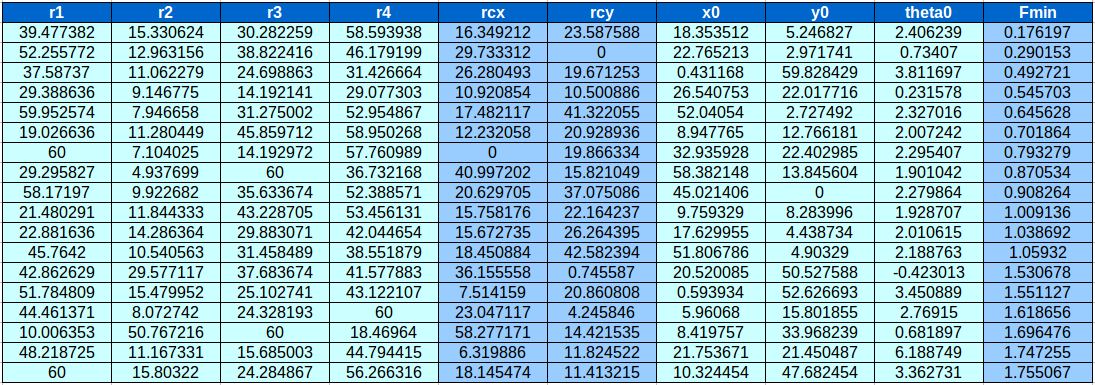
\includegraphics[width = 1.0\textwidth]{tabla.png}
    \caption{Tabla 1. Resultados preliminares.}
  \end{figure*}

    \begin{figure*}[ht]
    \center
    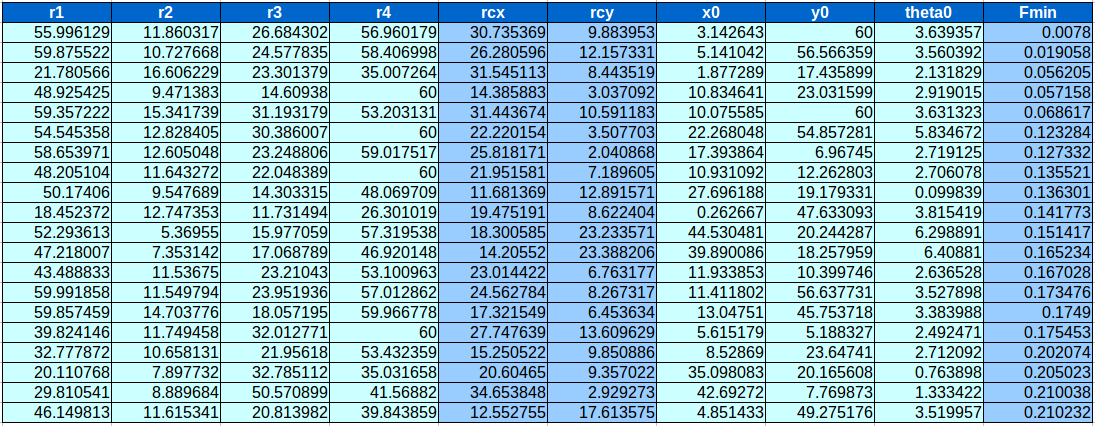
\includegraphics[width = 1.0\textwidth]{tabla2.png}
    \caption{Tabla 2. Resultados mejorados.}
  \end{figure*}
  
\subsubsection{Recombinaci\'on}

La recombinaci\'on puede deninirse como un proceso en el cual un conjunto $S_{par}$ de $n$ configuraciones (padres) se manipula para crear otro conjunto $S_{desc} \subseteq sol_P (x)$ de $m$ nuevas configuraciones (descendientes).\\

La generaci\'on de estos descendientes involucra la identificaci\'on y combinaci\'on de caracter\'isticas extra\'idas de los padres y transmitidas a la descendencia. En esta implemetaci\'on se utiliza un m\'etodo de recombinaci\'on denominado \emph{Dynastically Optimal Recombination} (DOR), en el cual cada recombinaci\'on posible es explorada para encontrar la configuraci\'on con mejor fitness, la consiguraci\'on obtenida ser\'a cuando menos tan buena como el mejor padre.\\

Adem\'as, estamos considerando una recombinaci\'on parcial, esto es, s\'olo se consideran ciertos bloques de informaci\'on en la recombinaci\'on de individuos; a saber, los conjuntos  $\{r_1,r_2,r_3,r_4\}$, $\{r_{cx},r_{cy}\}$, $\{x_0,y_0,\theta_0\}$ y $\{\theta_2^1,\theta_2^2,...,\theta_2^N\}$\\

\subsubsection{Mutatci\'on}

En la mutaci\'on, se crea un individuo $x'_i$ a partir de cada padre $x_i$, $\forall i \in \{1,2,...,popsize\}$ por medio de
 $$x'_i(j)=x_i(j)+\epsilon N_j(0,1)$$
 donde $j$ es un entero aleatorio $\in \{1,2,...,popsize\}$, y $N_j(0,1)$ es un valor aleatorio generado a partir de una distribuci\'on normal est\'andar. La constante $\epsilon$ es el radio de b\'usqueda local ya mencionado anteriormente.\\
 
 \begin{figure*}    
\begin{minipage}[t]{0.45\textwidth}
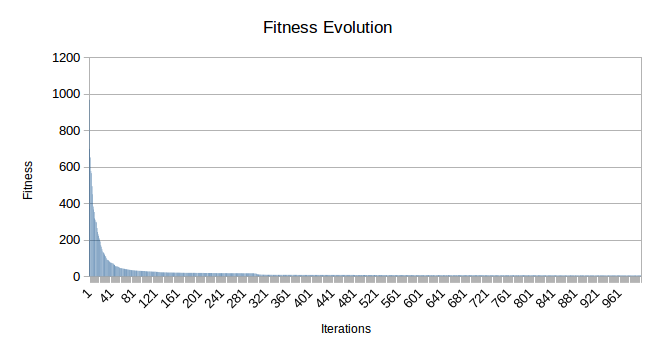
\includegraphics[width=\linewidth]{fitness1.png}
\caption{Figura 1. Evolución del fitness del algoritmo con recombinaci\'on DOR.}
\label{fig:immediate}
\end{minipage}
\hspace{\fill}
\begin{minipage}[t]{0.45\textwidth}
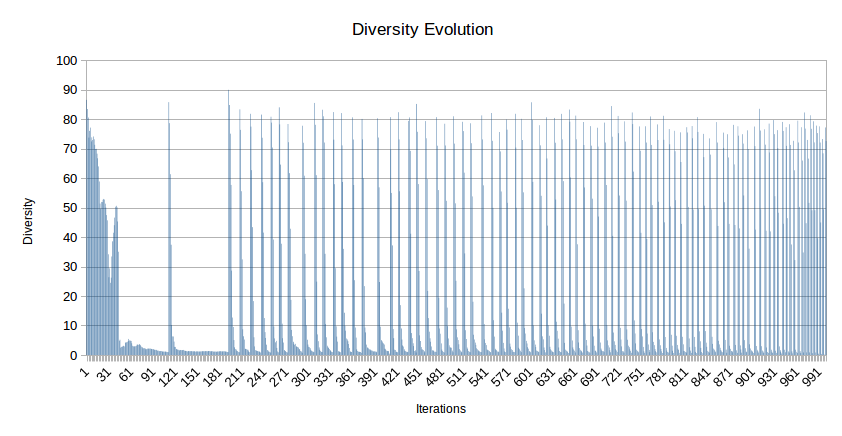
\includegraphics[width=\linewidth]{diversity1.png}
\caption{Figura 2. Evolución de la desviación estándar de la población con recombinaci\'on DOR.}
\label{fig:proximal}
\end{minipage}

\begin{minipage}[t]{0.45\textwidth}
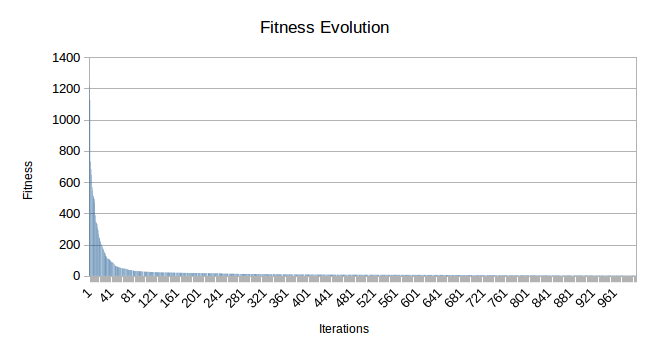
\includegraphics[width=\linewidth]{fitness2.png}
\caption{Figura 3. Evolución del fitness del algoritmo con recombinaci\'on aleatoria.}
\label{fig:distal}
\end{minipage}
\hspace{\fill}
\begin{minipage}[t]{0.45\textwidth}
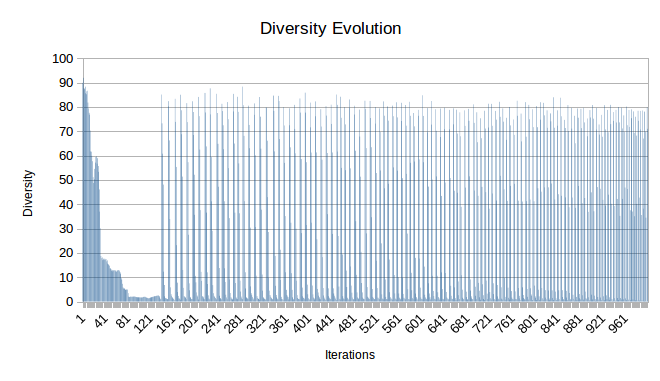
\includegraphics[width=\linewidth]{diversity2.png}
\caption{Figura 4. Evolución de la desviación estándar de la población con recombinaci\'on aleatoria.}
\label{fig:combined}
\end{minipage}

\end{figure*}

\section{Resultados}

\subsection{Preliminares}

La Tabla 1 muestra los mejores resultados obtenidos después de una prueba preliminar de 100 ejecuciones del algoritmo, se consideran las siguientes especificaciones:\\ 

 Puntos de precisi\'on: 
 $$C_d^i=\{(20,20),(20,25),(20,30),(20,35),(20,40),(20,45)\}$$
 L\'imites: $r_1,r_2,r_3,r_4,r_{cx},r_{cy},x_0,y_0 \in [0,60]$\\
 $\theta_0,\theta_2^1,\theta_2^2,\theta_2^3,\theta_2^4,\theta_2^5,\theta_2^6 \in [0,2\pi]$\\
 Par\'ametros:
 $popsize=100$, $MaxIte=1000$, $\epsilon_r=10$, $\epsilon_{\theta}=0.1$\\
 
\subsection{Mejoras}

Se hicieron dos modificaciones principales al algoritmo originalmente implementado:

\begin{enumerate}
	\item Se implement\'o un esquema adaptativo en la búsqueda local, el cual consiste en iniciar con un valor máximo de $\epsilon$ y conforme aumenta el numero de iteraciones, este valor se va decrementando, la idea es lograr una reducción del radio de búsqueda para incrementar la intensificación en la ultimas evaluaciones del algoritmo.
	\item Se combinaron dos esquemas de recombinaci\'on para cada mitad del numero total de iteraciones, durante la primera mitad se sigue un esquema aleatorio, esto es, se elige aleatoriamente una recombinaci\'on de todas las posibles; este esquema se incluy\'o con el propósito de mantener la diversidad durante las primeras etapas del algoritmo. Después de transcurrida la primera mitad de las iteraciones del algoritmo, se cambia este operador a un esquema dinástico, tal como se definió anteriormente.
\end{enumerate}

Las figuras 1-4 muestran el comportamiento del algoritmo considerando una recombinaci\'on DOR y una recombinaci\'on mixta, en la parte de la evolución del fitness, se muestra como al utilizar recombinaci\'on aleatoria al inicio, retrasa la necesidad del primer reinicio de la poblaci\'on, la cual toma lugar cuando la desviación estándar de la población cae por debajo de 1.


La Tabla 2 muestra los resultados mejorados después de implementar estas modificaciones. Puesto que para el caso de prueba implementado, el art\'iculo (referencia [1]) en el que nos estamos basando solamente proporciona el valor mínimo que se obtuvo (0.0267), s\'olo podemos concluir que nuestra implmentaci\'on fue capaz de producir un mejor resultado mínimo que el algoritmo propuesto en [1]. A continuaci\'on se muestra tambi\'en una estad\'istica que se obtuvo durante un total de 282 ejecuciones del programa:

   \begin{figure}[H]
    \centering
    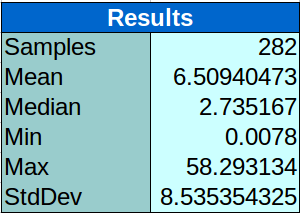
\includegraphics[width = 0.2\textwidth]{tablita.png}
    \caption{Estad\'isticas de las ejecuciones realizadas}
  \end{figure}
  
  
\section{Conclusiones}

Primero, se observ\'o durante la pr\'actica que no era posible utilizar un esquema demasiado enfocado en diversidad, puesto que se deseaba llegar al mínimo en un limite de 1000 iteraciones, por tanto, conven\'ia  contar con un esquema m\'as \emph{greedy} que nos permitiera alcanzar un mínimo en el menor tiempo posible.\\

También se pudo percibir durante la implmentaci\'on la diferencia que radica en aplicar una metaheur\'istica a un problema de optimizaci\'on continua, sobretodo aplicado a un problema donde se presentan muchas restricciones, y se observo que resulta ser una buena estrategia implementar una b\'usqueda local con alcance variable, ya que nos permite irnos enfocando en la intensificaci\'on de la soluci\'on a medida que el algoritmo avanza hacia un m\'inimo.

\section{Compilaci\'on-Ejecuci\'on}

Los programas implementados incluyen un makefile para compilarse, que soporta los comandos \emph{make}, \emph{make run} y \emph{make clean}, así como un script  de ejecución en el cluster.\\

\subsection{Programa de C\'alculos}

El programa de cálculos recibe como parámetros el tama\~no $N$ de la población, el numero máximo de iteraciones $MaxIte$, el archivo de entrada, que debe contener el numero de puntos de precision que se van a optimizar y las coordenadas (x,y) de esos puntos, y por \'ultimo, el archivo de salida donde se va a guardar el resultado.

   \begin{figure}[H]
    \centering
    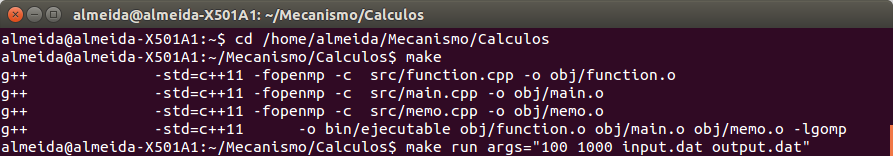
\includegraphics[width = 0.5\textwidth]{screen1.png}
    \caption{Compilaci\'on y ejecuci\'on del programa de c\'alculos.}
  \end{figure}

\subsection{Programa de Simulaci\'on}
El programa de simulación lee el archivo de entrada y el archivo de salida generado por el programa de cálculos para correr la simulación del mecanismo (Se requiere WxWidgets). Recibe como parámetros el directorio de estos archivos (Se incluyen visualizaciones de algunos resultados obtenidos).

   \begin{figure}[H]
    \centering
    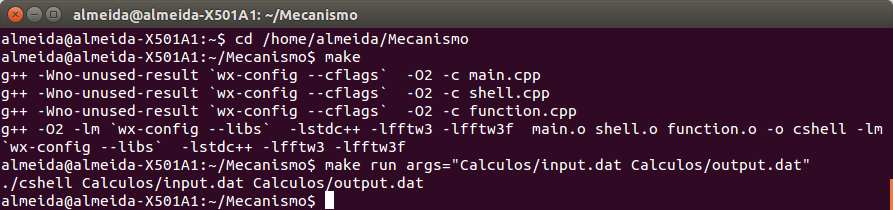
\includegraphics[width = 0.5\textwidth]{screen2.png}
    \caption{Compilaci\'on y ejecuci\'on del simulador.}
  \end{figure}

   \begin{figure}[H]
    \centering
    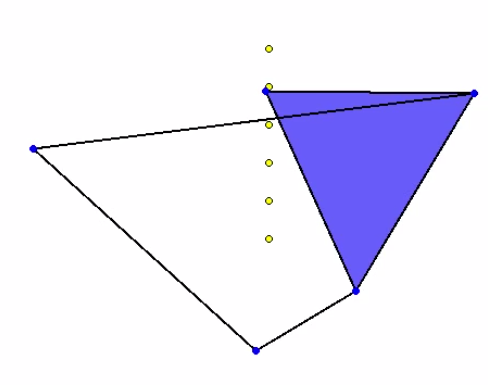
\includegraphics[width = 0.5\textwidth]{simulacion.png}
    \caption{Simulaci\'on del Mecanismo.}
  \end{figure}
  
\section{Referencias}


\bibliographystyle{plainnat}


\begin{itemize}

\begin{small}

\item[1]
{\it J.A. Cabrera \& A. Simon, M. Prado} (2002).
{\bf Optimal synthesis of mechanisms with genetic algorithms.} Journal of Mechanism and Machine Theory 37 (2002) 1165-1177.

\vspace{0.2cm}

\item[2]
{\it El-Ghazali Talbi} (2009).
{\bf Metaheuristics: form Design to Implementation.} John Wiley \& Sons, Inc.

\vspace{0.2cm}

\item[3]
{\it Pablo Moscato \& Carlos Cotta} (2003).
{\bf A Gentle Introduction to Memetic Algorithms.} Handbook of Metaheuristics, Kluwer
Academic Publishers, pp. 105-144

\vspace{0.2cm}

\item[4]
{\it Kumar Chellapilla} (1998).
{\bf Combining Mutation Operators in Evolutionary Programming.} IEEE Transactions on Evolutionary Computation, Vol. 2, No. 3.

\vspace{0.2cm}

\item[5]
{\it Ferrante Neri \& Carlos Cotta} (2012).
{\bf Memetic algorithms and memetic computing optimization: A literature review.} Swarm and Evolutionary Computation 2, 1–14.

\end{small}
\end{itemize}

\end{document}


